\documentclass[tikz, border=12pt]{standalone}

\usepackage{tikz}
\usetikzlibrary{
  shapes.geometric,
  shapes.misc,
  arrows.meta,
  positioning,
  fit,
  backgrounds,
  calc
}
\usepackage[T1]{fontenc}
\usepackage{lmodern}
\usepackage{amssymb}

%% ── Thesis colour palette ────────────────────────────────────
\definecolor{navyblue}{RGB}{31,78,121}
\definecolor{navylight}{RGB}{52,114,168}
\definecolor{slategray}{RGB}{100,120,140}
\definecolor{boxbg}{RGB}{235,242,250}
\definecolor{boxborder}{RGB}{180,210,240}
\definecolor{arrowgray}{RGB}{80,100,120}
\definecolor{labelgray}{RGB}{60,80,100}
\definecolor{forestgreen}{RGB}{34,100,60}
\definecolor{forestbg}{RGB}{230,245,235}
\definecolor{domainbg}{RGB}{220,235,250}
\definecolor{oubg}{RGB}{235,235,255}
\definecolor{oucolor}{RGB}{70,70,180}
\definecolor{objbg}{RGB}{250,250,250}

%% ── Circled step number ──────────────────────────────────────
\newcommand{\stepnum}[1]{%
  \tikz[baseline=(n.base)]\node[circle,
    draw=navyblue, fill=navyblue, text=white,
    font=\scriptsize\bfseries,
    inner sep=1.5pt, minimum size=0.5cm] (n) {#1};}

%% ── Common styles ────────────────────────────────────────────
\tikzset{
  forestbox/.style={
    draw=forestgreen, fill=forestbg, line width=1.2pt,
    rounded corners=5pt, minimum width=3.2cm,
    minimum height=0.85cm, align=center,
    font=\small\bfseries\color{forestgreen}
  },
  domainbox/.style={
    draw=navyblue, fill=domainbg, line width=1.0pt,
    rounded corners=4pt, minimum width=2.8cm,
    minimum height=0.8cm, align=center,
    font=\small\bfseries\color{navyblue}
  },
  oubox/.style={
    draw=oucolor, fill=oubg, line width=0.8pt,
    rounded corners=3pt, minimum width=2.4cm,
    minimum height=0.7cm, align=center,
    font=\small\color{oucolor}
  },
  objbox/.style={
    draw=slategray, fill=objbg, line width=0.6pt,
    rounded corners=2pt, minimum width=1.9cm,
    minimum height=0.65cm, align=center,
    font=\scriptsize\color{labelgray}
  },
  entitybox/.style={
    draw=navyblue, fill=domainbg, line width=1.2pt,
    rounded corners=5pt, minimum width=2.4cm,
    minimum height=1.1cm, align=center,
    font=\small\bfseries\color{navyblue}
  },
  msgbox/.style={
    draw=boxborder, fill=boxbg, line width=0.8pt,
    rounded corners=3pt,
    font=\scriptsize\color{labelgray},
    inner sep=5pt, align=left
  },
  thesisarrow/.style={
    -{Stealth[length=6pt,width=4pt]},
    draw=arrowgray, line width=1.0pt
  },
  dasharrow/.style={
    -{Stealth[length=5pt,width=3.5pt]},
    draw=arrowgray, dashed, line width=0.9pt
  },
  bidiarrow/.style={
    {Stealth[length=5pt,width=3.5pt]}-{Stealth[length=5pt,width=3.5pt]},
    draw=arrowgray, line width=1.0pt
  },
  arrowlabel/.style={
    font=\scriptsize\color{labelgray},
    fill=white, inner sep=2pt
  },
  diagramtitle/.style={
    font=\large\bfseries\color{navyblue}
  },
}

\begin{document}

%% ============================================================
%%  DIAGRAM 1 — AD Object Hierarchy
%% ============================================================
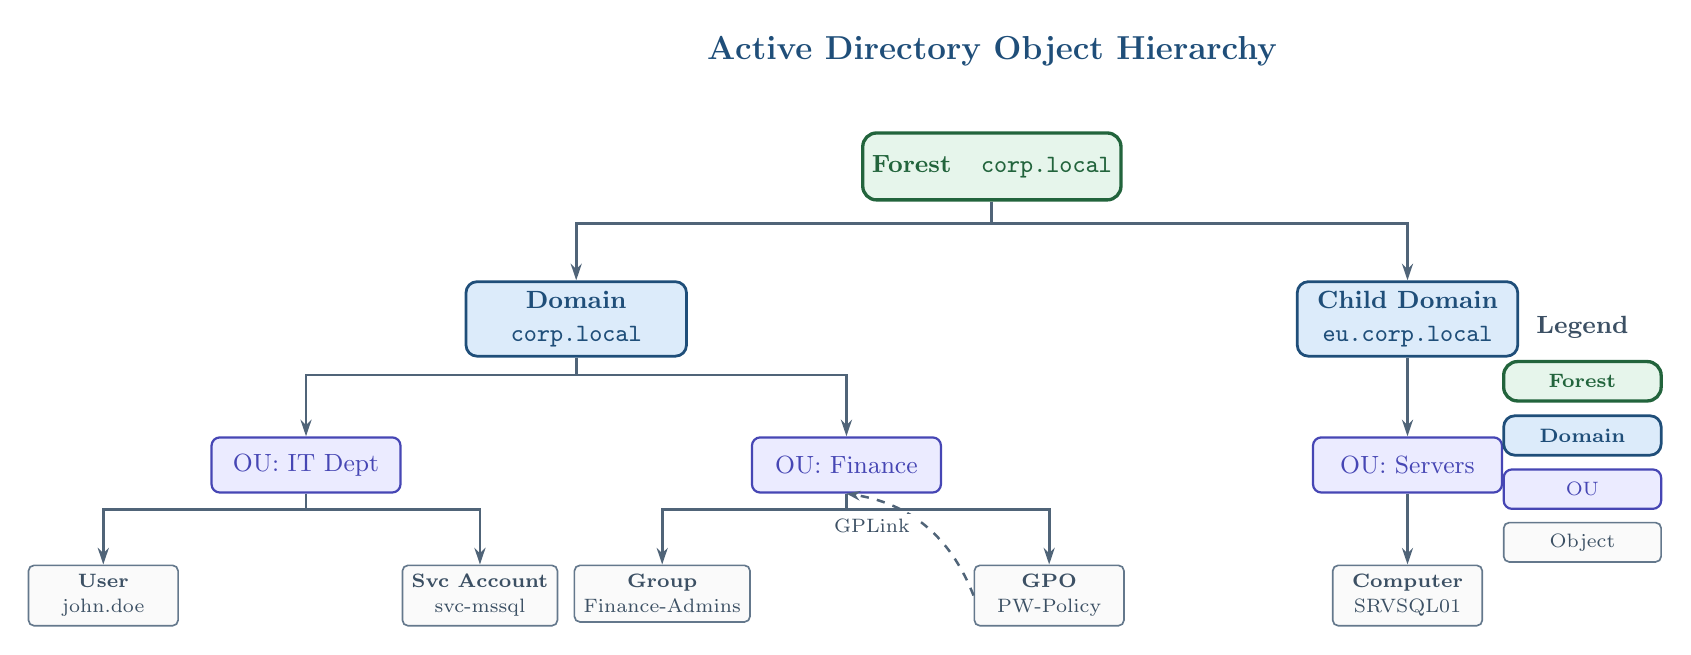
\begin{tikzpicture}[node distance=0.5cm and 0.5cm]

  \node[diagramtitle] (T) {Active Directory Object Hierarchy};

  %% Forest
  \node[forestbox, below=0.7cm of T] (forest)
    {Forest\quad\texttt{corp.local}};

  %% Domains
  \node[domainbox, below left=1.0cm and 2.2cm of forest] (d1)
    {Domain\\[1pt]\texttt{corp.local}};
  \node[domainbox, below right=1.0cm and 2.2cm of forest] (d2)
    {Child Domain\\[1pt]\texttt{eu.corp.local}};

  \draw[thesisarrow] (forest.south) -- ++(0,-0.28) -| (d1.north);
  \draw[thesisarrow] (forest.south) -- ++(0,-0.28) -| (d2.north);

  %% OUs under d1
  \node[oubox, below left=1.0cm and 0.8cm of d1] (ou1) {OU: IT Dept};
  \node[oubox, below right=1.0cm and 0.8cm of d1] (ou2) {OU: Finance};

  \draw[thesisarrow] (d1.south) -- ++(0,-0.22) -| (ou1.north);
  \draw[thesisarrow] (d1.south) -- ++(0,-0.22) -| (ou2.north);

  %% OU under d2
  \node[oubox, below=1.0cm of d2] (ou3) {OU: Servers};
  \draw[thesisarrow] (d2.south) -- (ou3.north);

  %% Objects under ou1
  \node[objbox, below left=0.9cm and 0.4cm of ou1] (u1)
    {\textbf{User}\\[1pt]john.doe};
  \node[objbox, below right=0.9cm and 0cm of ou1] (s1)
    {\textbf{Svc Account}\\[1pt]svc-mssql};

  \draw[thesisarrow] (ou1.south) -- ++(0,-0.2) -| (u1.north);
  \draw[thesisarrow] (ou1.south) -- ++(0,-0.2) -| (s1.north);

  %% Objects under ou2
  \node[objbox, below left=0.9cm and 0cm of ou2] (g1)
    {\textbf{Group}\\[1pt]Finance-Admins};
  \node[objbox, below right=0.9cm and 0.4cm of ou2] (gpo)
    {\textbf{GPO}\\[1pt]PW-Policy};

  \draw[thesisarrow] (ou2.south) -- ++(0,-0.2) -| (g1.north);
  \draw[thesisarrow] (ou2.south) -- ++(0,-0.2) -| (gpo.north);

  %% Objects under ou3
  \node[objbox, below=0.9cm of ou3] (c1)
    {\textbf{Computer}\\[1pt]SRVSQL01};
  \draw[thesisarrow] (ou3.south) -- (c1.north);

  %% GPLink dashed
  \draw[dasharrow, bend right=30] (gpo.west)
    to node[arrowlabel, left=3pt] {GPLink} (ou2.south);

  %% Legend
  \begin{scope}[shift={(7.5,-3.5)}]
    \node[font=\small\bfseries\color{labelgray}] (lt) {Legend};
    \node[forestbox, minimum width=2.0cm, minimum height=0.5cm,
          font=\scriptsize\bfseries\color{forestgreen},
          below=0.15cm of lt] (ll1) {Forest};
    \node[domainbox, minimum width=2.0cm, minimum height=0.5cm,
          font=\scriptsize\bfseries\color{navyblue},
          below=0.15cm of ll1] (ll2) {Domain};
    \node[oubox, minimum width=2.0cm, minimum height=0.5cm,
          font=\scriptsize\color{oucolor},
          below=0.15cm of ll2] (ll3) {OU};
    \node[objbox, minimum width=2.0cm, minimum height=0.5cm,
          below=0.15cm of ll3] (ll4) {Object};
  \end{scope}

\end{tikzpicture}

%% ============================================================
%%  DIAGRAM 2 — Forest and Trust Relationships
%% ============================================================
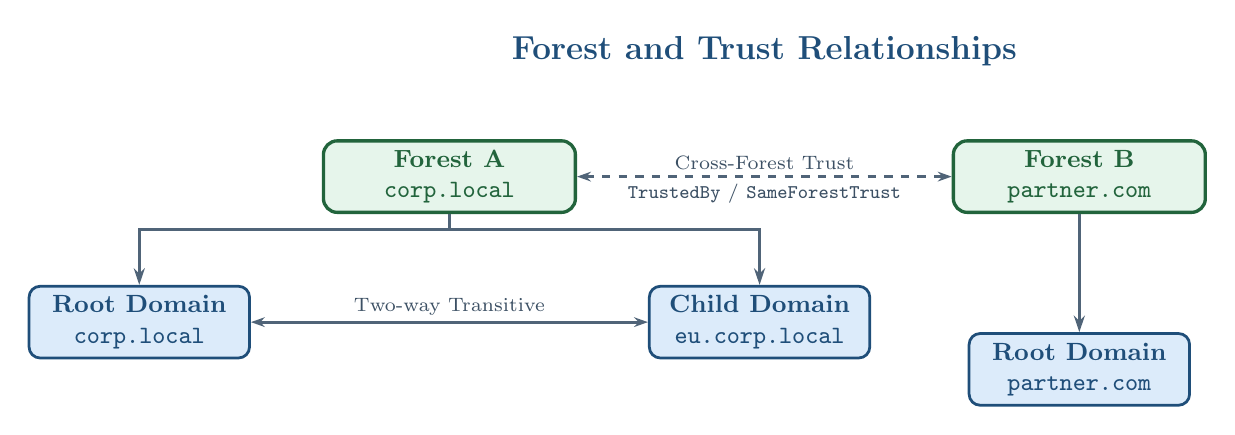
\begin{tikzpicture}[node distance=0.9cm and 1.8cm]

  \node[diagramtitle] (T) {Forest and Trust Relationships};

  %% Forest A
  \node[forestbox, below=0.8cm of T, xshift=-4.0cm] (fA)
    {Forest A\\\texttt{corp.local}};
  \node[domainbox, below left=0.9cm and 0.9cm of fA] (dA1)
    {Root Domain\\\texttt{corp.local}};
  \node[domainbox, below right=0.9cm and 0.9cm of fA] (dA2)
    {Child Domain\\\texttt{eu.corp.local}};

  \draw[thesisarrow] (fA.south) -- ++(0,-0.2) -| (dA1.north);
  \draw[thesisarrow] (fA.south) -- ++(0,-0.2) -| (dA2.north);

  \draw[bidiarrow] (dA1.east) -- (dA2.west)
    node[arrowlabel, above, midway] {Two-way Transitive};

  %% Forest B
  \node[forestbox, below=0.8cm of T, xshift=4.0cm] (fB)
    {Forest B\\\texttt{partner.com}};
  \node[domainbox, below=1.5cm of fB] (dB1)
    {Root Domain\\\texttt{partner.com}};
  \draw[thesisarrow] (fB.south) -- (dB1.north);

  %% Cross-forest trust
  \draw[bidiarrow, dashed]
    (fA.east) -- (fB.west)
    node[arrowlabel, above, midway] {Cross-Forest Trust}
    node[arrowlabel, below, midway] {\texttt{TrustedBy} / \texttt{SameForestTrust}};

  %% Annotation
%  \node[msgbox, below=3.5cm of T, minimum width=7.5cm] (note) {
%    \textbf{BloodHound edge naming inconsistency:} SharpHound versions\\
%    differ in how they label trust edges (\texttt{TrustedBy} vs.\\
%    \texttt{SameForestTrust}). Both are aliased in \texttt{build\_dataset.py}.
%  };

\end{tikzpicture}

%% ============================================================
%%  DIAGRAM 3 — LDAP Query Flow
%% ============================================================
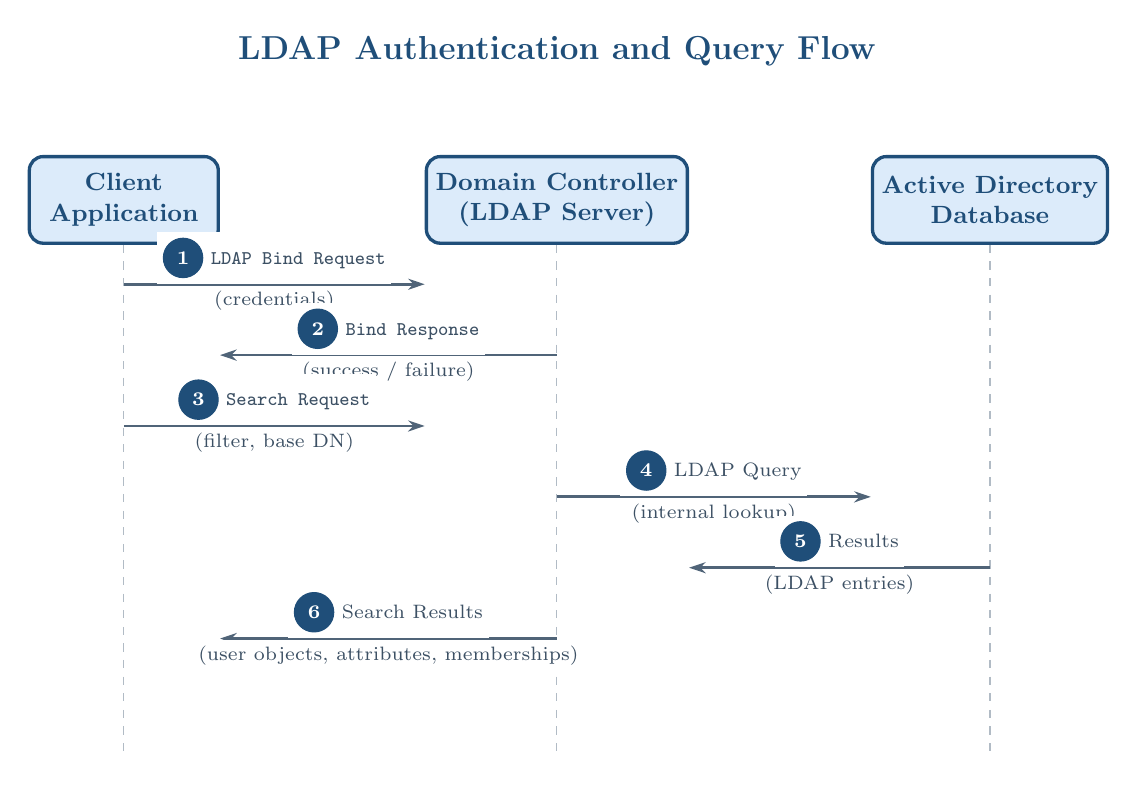
\begin{tikzpicture}[node distance=2.0cm and 0.8cm]

  \node[diagramtitle] (T) {LDAP Authentication and Query Flow};

  %% Entities — horizontal layout
  \node[entitybox, below=1.0cm of T, xshift=-5.5cm] (cli)
    {Client\\Application};
  \node[entitybox, below=1.0cm of T] (dc)
    {Domain Controller\\(LDAP Server)};
  \node[entitybox, below=1.0cm of T, xshift=5.5cm] (adb)
    {Active Directory\\Database};

  %% Vertical lifelines
  \draw[draw=slategray!50, dashed, thin]
    (cli.south) -- ++(0,-6.5);
  \draw[draw=slategray!50, dashed, thin]
    (dc.south) -- ++(0,-6.5);
  \draw[draw=slategray!50, dashed, thin]
    (adb.south) -- ++(0,-6.5);

  %% Messages
  %% 1 Bind REQ client→dc
  \draw[thesisarrow]
    ([yshift=-0.5cm]cli.south) -- ([yshift=-0.5cm]dc.south west |- cli.south)
    node[arrowlabel, above, midway] {\stepnum{1}~\texttt{LDAP Bind Request}}
    node[arrowlabel, below, midway] {(credentials)};

  %% 2 Bind RESP dc→client
  \draw[thesisarrow]
    ([yshift=-1.4cm]dc.south) -- ([yshift=-1.4cm]cli.south east |- dc.south)
    node[arrowlabel, above, midway] {\stepnum{2}~\texttt{Bind Response}}
    node[arrowlabel, below, midway] {(success / failure)};

  %% 3 Search REQ client→dc
  \draw[thesisarrow]
    ([yshift=-2.3cm]cli.south) -- ([yshift=-2.3cm]dc.south west |- cli.south)
    node[arrowlabel, above, midway] {\stepnum{3}~\texttt{Search Request}}
    node[arrowlabel, below, midway] {(filter, base DN)};

  %% 4 LDAP query dc→AD
  \draw[thesisarrow]
    ([yshift=-3.2cm]dc.south) -- ([yshift=-3.2cm]adb.south west |- dc.south)
    node[arrowlabel, above, midway] {\stepnum{4}~LDAP Query}
    node[arrowlabel, below, midway] {(internal lookup)};

  %% 5 Results AD→dc
  \draw[thesisarrow]
    ([yshift=-4.1cm]adb.south) -- ([yshift=-4.1cm]dc.south east |- adb.south)
    node[arrowlabel, above, midway] {\stepnum{5}~Results}
    node[arrowlabel, below, midway] {(LDAP entries)};

  %% 6 Results dc→client
  \draw[thesisarrow]
    ([yshift=-5.0cm]dc.south) -- ([yshift=-5.0cm]cli.south east |- dc.south)
    node[arrowlabel, above, midway] {\stepnum{6}~Search Results}
    node[arrowlabel, below, midway] {(user objects, attributes, memberships)};

  %% Note
%  \node[msgbox, below=6.5cm of T, xshift=-5.5cm,
%        minimum width=12.0cm, align=left] {
%    \textbf{Role in BloodHound collection:}
%    LDAP is used by SharpHound and \texttt{bloodhound-python} to enumerate
%    all AD objects, group memberships, ACLs, and GPO links.
%    Every node and edge in the attack graph originates from LDAP query results.
%  };

\end{tikzpicture}

%% ============================================================
%%  DIAGRAM 4 — Kerberos Authentication Flow
%% ============================================================
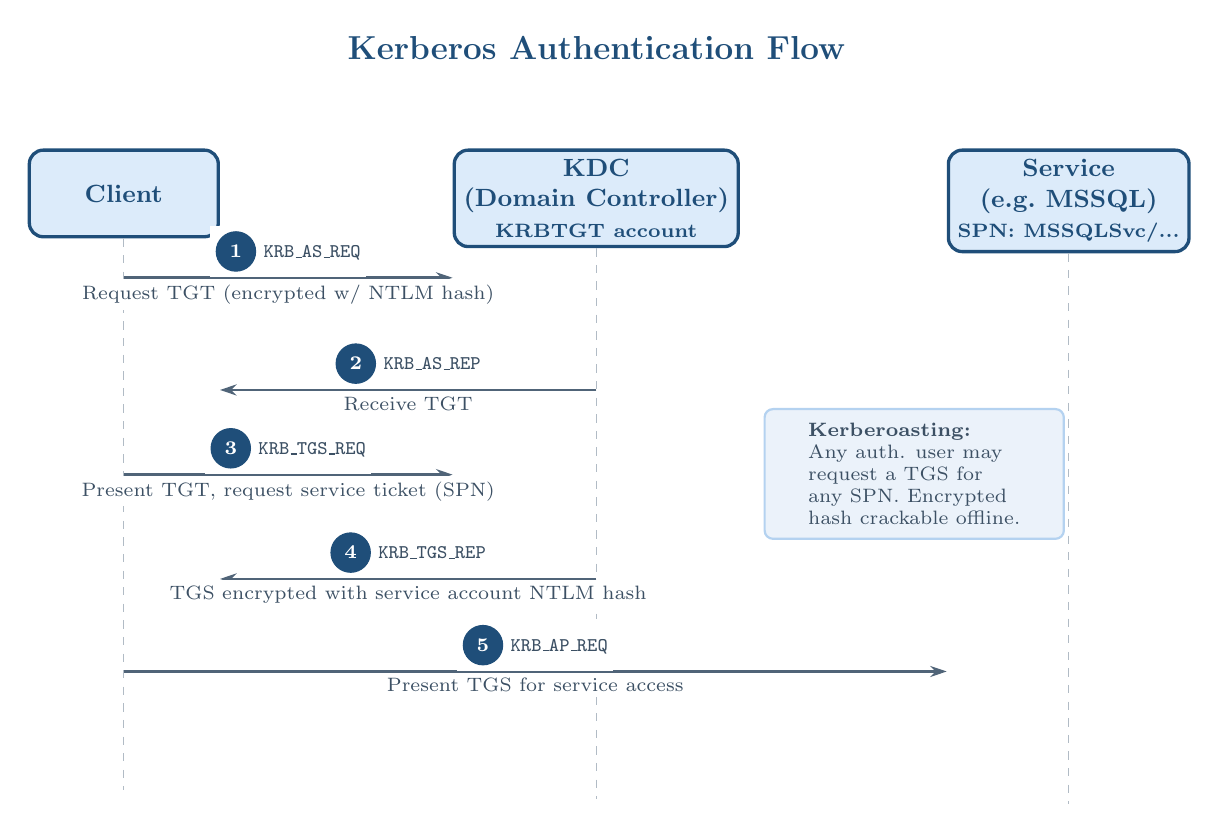
\begin{tikzpicture}[node distance=2.5cm and 0.8cm]

  \node[diagramtitle] (T) {Kerberos Authentication Flow};

  %% Entities
  \node[entitybox, below=1.0cm of T, xshift=-6.0cm] (kc)
    {Client};
  \node[entitybox, below=1.0cm of T] (kdc)
    {KDC\\(Domain Controller)\\{\scriptsize KRBTGT account}};
  \node[entitybox, below=1.0cm of T, xshift=6.0cm] (ksvc)
    {Service\\(e.g.\ MSSQL)\\{\scriptsize SPN: MSSQLSvc/...}};

  %% Lifelines
  \draw[draw=slategray!50, dashed, thin]
    (kc.south) -- ++(0,-7.0);
  \draw[draw=slategray!50, dashed, thin]
    (kdc.south) -- ++(0,-7.0);
  \draw[draw=slategray!50, dashed, thin]
    (ksvc.south) -- ++(0,-7.0);

  %% 1 AS-REQ
  \draw[thesisarrow]
    ([yshift=-0.5cm]kc.south) -- ([yshift=-0.5cm]kdc.south west |- kc.south)
    node[arrowlabel, above, midway] {\stepnum{1}~\texttt{KRB\_AS\_REQ}}
    node[arrowlabel, below, midway] {Request TGT (encrypted w/ NTLM hash)};

  %% 2 AS-REP
  \draw[thesisarrow]
    ([yshift=-1.8cm]kdc.south) -- ([yshift=-1.8cm]kc.south east |- kdc.south)
    node[arrowlabel, above, midway] {\stepnum{2}~\texttt{KRB\_AS\_REP}}
    node[arrowlabel, below, midway] {Receive TGT};

  %% 3 TGS-REQ
  \draw[thesisarrow]
    ([yshift=-3cm]kc.south) -- ([yshift=-3cm]kdc.south west |- kc.south)
    node[arrowlabel, above, midway] {\stepnum{3}~\texttt{KRB\_TGS\_REQ}}
    node[arrowlabel, below, midway] {Present TGT, request service ticket (SPN)};

  %% 4 TGS-REP
  \draw[thesisarrow]
    ([yshift=-4.2cm]kdc.south) -- ([yshift=-4.2cm]kc.south east |- kdc.south)
    node[arrowlabel, above, midway] {\stepnum{4}~\texttt{KRB\_TGS\_REP}}
    node[arrowlabel, below, midway] {TGS encrypted with service account NTLM hash};

  %% 5 AP-REQ client→service
  \draw[thesisarrow]
    ([yshift=-5.5cm]kc.south) -- ([yshift=-5.5cm]ksvc.south west |- kc.south)
    node[arrowlabel, above, midway] {\stepnum{5}~\texttt{KRB\_AP\_REQ}}
    node[arrowlabel, below, midway] {Present TGS for service access};

  %% Annotation: Kerberoasting
  \node[msgbox, right=0.3cm of kdc, yshift=-3.5cm,
        minimum width=3.8cm] {
    \textbf{Kerberoasting:}\\
    Any auth. user may\\
    request a TGS for\\
    any SPN. Encrypted\\
    hash crackable offline.
  };

  %% Offensive note bottom
%  \node[msgbox, below=5.8cm of T, xshift=-6.0cm,
%        minimum width=13.0cm, align=left] {
%    \textbf{Offensive relevance in this thesis:}
%    \textbf{Constrained delegation} (\texttt{AllowedToDelegate}): a service may
%    request a TGS on behalf of any user, enabling privilege escalation chains
%    captured as \texttt{allowedtodelegate} edges in the pipeline.
%    \textbf{DCSync} bypasses Kerberos entirely: it abuses replication rights
%    (\texttt{GetChanges} + \texttt{GetChangesAll}) to extract all NTLM hashes
%    from the domain controller directly --- no ticket exchange required.
%  };

\end{tikzpicture}

\end{document}